\documentclass[10pt,xcolor=pdflatex,hyperref={unicode}]{beamer}
\usepackage{newcent}
\usepackage[utf8]{inputenc}
%\usepackage[czech]{babel}
%\usepackage[T1]{fontenc}
\usepackage{hyperref}
\usepackage{fancyvrb}
\usetheme{FIT}

\usepackage{setspace}
\usepackage{enumerate}
\usepackage[export]{adjustbox}
\usepackage{wrapfig}
%%%%%%%%%%%%%%%%%%%%%%%%%%%%%%%%%%%%%%%%%%%%%%%%%%%%%%%%%%%%%%%%%%
\title{Block Cleaning Application\\
(an10)}

\author[]{
Beránek Tomáš, Buchta Martin,\\
Klem Richard, Pešková Daniela}

\institute[]{Brno University of Technology, Faculty of Information Technology\\
Bo\v{z}et\v{e}chova 1/2. 612 66 Brno - Kr\'alovo Pole}


% České logo - Czech logo
% beamerouterthemeFIT.sty řádek 9: fitlogo1_cz

\date{\today}
%\date{} % bez data / without date

%%%%%%%%%%%%%%%%%%%%%%%%%%%%%%%%%%%%%%%%%%%%%%%%%%%%%%%%%%%%%%%%%%

\begin{document}


\frame[plain]{\titlepage}


\begin{frame}\frametitle{Motivation}
    \begin{itemize}
        \item Fine for removing a vehicle.
        \vspace{0.25cm}
        \item Lack of block cleaning signs.
        \vspace{0.25cm}
        \item Block cleaning dates must be sought for each Brno district \emph{separately}.
    \end{itemize}
    
    \begin{center}
        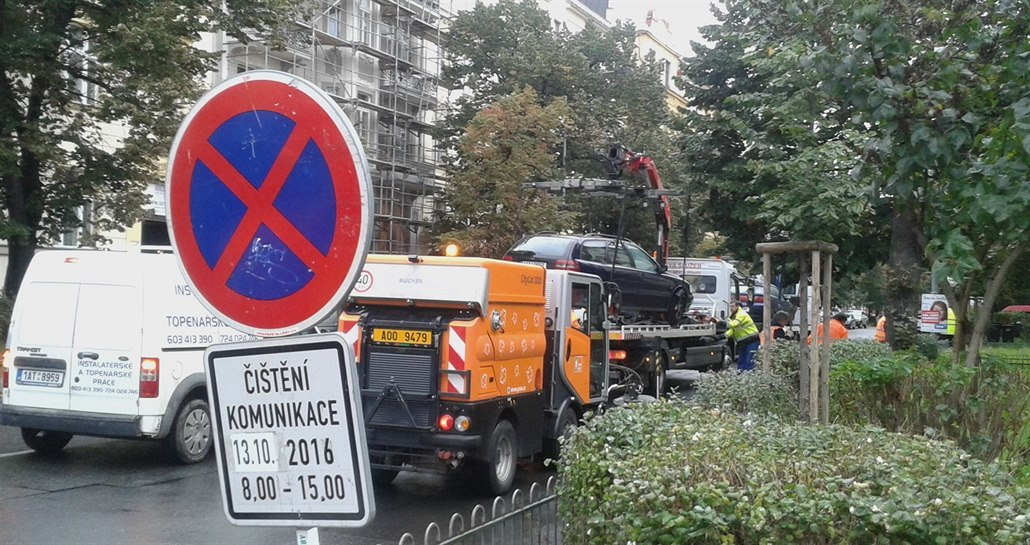
\includegraphics[width=0.65\paperwidth]{img/block-cleaning-1.jpg}
    \end{center}
\end{frame}


\begin{frame}\frametitle{Possible Development Problems}
    \doublespacing
    \begin{itemize}
        \item Using \emph{Web scraping} to retrieve dates of block cleaning.
        \item Using \emph{dynamic maps}:
            \begin{itemize}
                \item \alert{Solution}: using Google Maps SDK for Android devices.
            \end{itemize}
            
        \item Permission to use \emph{GPS}:
            \begin{itemize}
                \item \alert{Solution}: possibility to use the app without GPS.
            \end{itemize}
    \end{itemize}
        
    \begin{figure}
        \centering
        \begin{minipage}{0.5\textwidth}
            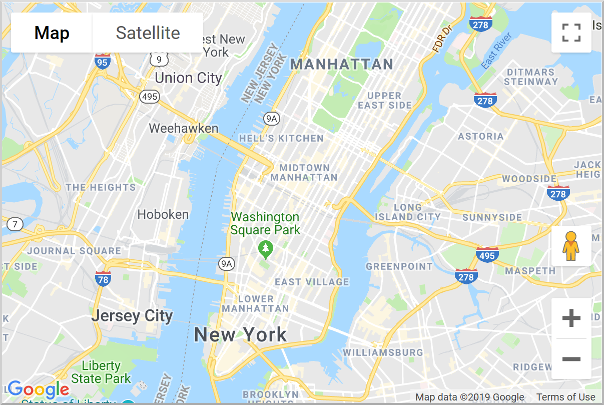
\includegraphics[width=0.5\paperwidth]{img/block-cleaning-2.png}
        \end{minipage}
        \hfill
        \begin{minipage}{0.35\textwidth}
            \raggedleft
            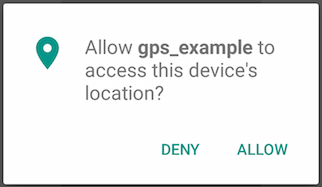
\includegraphics[width=0.3\paperwidth]{img/block-cleaning-3.png}
        \end{minipage}
    \end{figure}
\end{frame}


\begin{frame}\frametitle{Wireframes}
    \begin{figure}
        \centering
        \begin{minipage}{0.3\textwidth}
            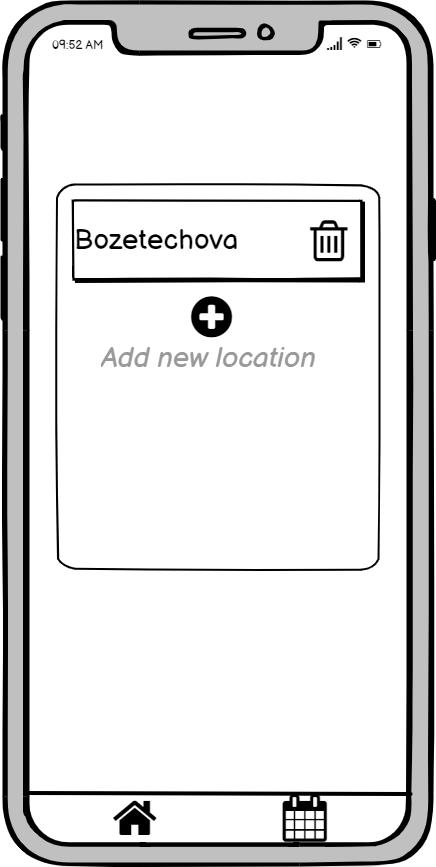
\includegraphics[width=0.25\paperwidth]{img/wireframe1.png}
        \end{minipage}
        \hfill
        \begin{minipage}{0.3\textwidth}
            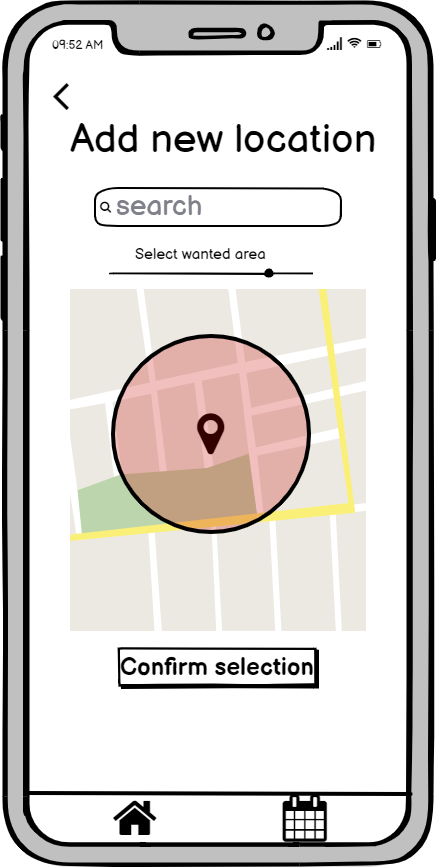
\includegraphics[width=0.25\paperwidth]{img/wireframe2.png}
        \end{minipage}
        \hfill
        \begin{minipage}{0.3\textwidth}
            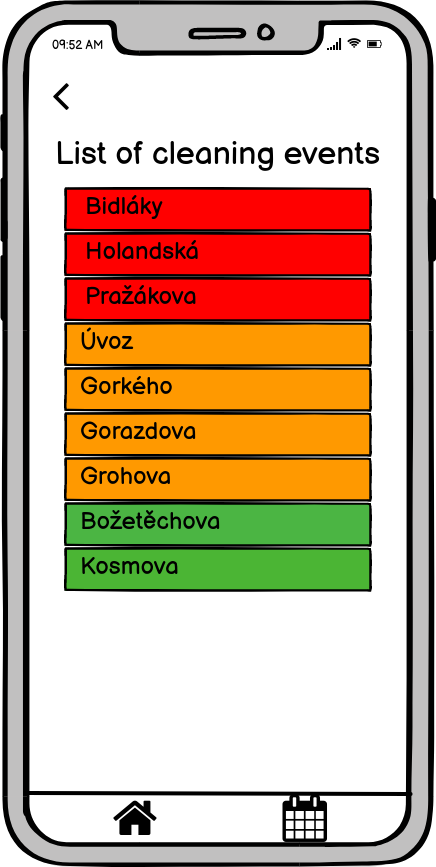
\includegraphics[width=0.25\paperwidth]{img/wireframe3.png}
        \end{minipage}
    \end{figure}
\end{frame}


\begin{frame}\frametitle{Similar Solutions}
    \doublespacing
    \begin{itemize}
        \item Only a single similar app was found -- \emph{Brněnské komunikace}.
        \item Rating 2.5/5 stars.
        \item Does not display all dates.
        \item Not possible to choose a single street to be monitored.
    \end{itemize}
    \vspace{0.25cm}
    
    \begin{center}
        
\includegraphics[width=0.75\paperwidth]{img/block-cleaning-4.png}
    \end{center}
\end{frame}


\begin{frame}\frametitle{Time Plan}
    \begin{itemize}
        \item[] \alert{Oct 4} -- wireframes, presentation for Project Workshop
        \item[] \alert{Oct 5} -- Project Workshop
        \item[] \alert{Oct 10} -- agreeing on the technologies to be used
        \item[] \alert{Oct 17} -- creating a basic UI
        \item[] \alert{Oct 26} -- Project Workshop
        \item[] \alert{Nov 7}  -- adding a dynamic map and web scraping
        \item[] \alert{Nov 14} -- functionality testing and documentation
        \item[] \alert{Nov 16} -- Project Workshop
        \item[] \alert{Dec 7}  -- Project Workshop
        \item[] \alert{Dec 12} -- project submission
        \item[] \alert{Dec 14} -- Project Workshop
    \end{itemize}
\end{frame}


\bluepage{Thank you for your attention}
\end{document}
